\chapter{Calculation of the Formation Energy of the [$Cu_{Zn}^- + Zn_{Cu}^+$] Defect Pair in {\CZTS}}\label{Cu-Zn_defects_calc}
The defect formation energy, $\Delta H_D$, is the main quantity of interest in the theoretical description of defects and impurities. It can be used to determine the defect concentrations in equilibrium, as shown in equation \ref{defect_conc}, and also the thermodynamic transition energies between different possible charge states of electrically active defects \cite{defects_Lany}. 
%The former will be discussed later in this section and the latter will be discussed further in relation to sulfur vacancies in {\CZTS} in section \ref{Vs_proj}. 
It is common to use the supercell method when performing simulations of defects in solid state systems. 
In this method, a defect is inserted into a larger supercell to screen interactions between defects across a boundary when implementing periodic boundary conditions. The supercell should be chosen to ensure that it is large enough to prevent interactions between point defects in adjacent cells. In practise, it is often too computationally expensive to meet this requirement completely as the number of atoms in the supercell rises with the third power of the linear size of the supercell and the computational expense then increases with the third power of the number of atoms \cite{supercell_method}. In our calculations of defects in {\CZTS} we use a 64 atom supercell, which is the most isotropic and largest supercell that could feasibly be used for our calculations at the level of accuracy we required. This corresponds to a cell size of approximately $11\times11\times11 \AA^3$. This supercell is constructed by creating a $2\times2\times1$ supercell of the conventional CZTS supercell shown in figure \ref{CZTS_cell}.

The full expression for the formation energy of a defect is given in equation \ref{defect_formation}, where $\Delta H_{D,q}$ is the total energy of the supercell containing the defect in charge state q, $E_H$ is the total energy of an equivalent supercell of the perfect host crystal without the defect. The chemical potential $\mu_{\alpha}$ describes the energy of the atomic reservoir of the atoms $\alpha$ removed from or added to the host crystal when the defect forms. For charged defects, where q $\neq$ 0, $E_F$ describes the energy of the reservoir of electrons, which is usually considered to be somewhere between the valence band maximum and conduction band minimum, but can be tuned by an applied bias.
However, in the case of the antisite pair [$Cu_{Zn}^- + Zn_{Cu}^+$], we do not add or remove any atoms, we only substitute their positions. Also the defect complex is overall charge neutral and so the full expression simplifies to that shown in equation \ref{defect_formation_reduced}.
\begin{equation} \label{defect_formation}
\Delta H_{D,q}(E_F, \mu) = [E_{D,q} - E_H] + \sum_\alpha n_{\alpha}\mu_{\alpha} + q \cdot E_F
\end{equation}
\begin{equation} \label{defect_formation_reduced}
\Delta H_{D} = E_{D,q} - E_H
\end{equation}

First principles calculations using the density function theory (DFT) formalism have been found to yield reliable information about atomic structure, including the relaxation of the host atoms, during the formation of a defect in a crystal. A brief overview of standard DFT methodology for the calculation of total energies is given in Appendix \ref{DFT_methods}. However, in many cases traditional DFT functionals used in standard DFT methods often fail at the description of the electronic structure of a defective crystal. For instance, the local density approximation (LDA) and generalized gradient approximation (GGA), severely underestimate the band gaps of semiconductors and insulators \cite{defects_tutorial}.
Defect formation energies are in general affected by this band-gap problem in two ways. Firstly, defect states may be predicted to be within the continuum of host states when the band gap is underestimated but actually be within the band gap if the band-gap problem is corrected. The result of this incorrect placement of the defect level is that electron-occupied defect states can erroneously spill into the conduction band or similarly hole defects could spill into the valence band. The calculated charge density associated with these defects would then be incorrect, resulting in an uncontrolled error in the value obtained for $\Delta H_{D,q}$. For charged defects, there is an additional source of error due to $\Delta H_{D,q}$ being dependent upon the Fermi level. $E_F$ is bounded by the bang-edge energies and so when the band gap is changed the range of formation energies between the valence band maximum and conduction band minimum is altered \cite{defects_Lany}.
The band gap problem can be addressed by going beyond DFT. One such method is hybrid-DFT. Hybrid approaches incorporate a certain amount of screened exact exchange from the Hartree-Fock approximation with DFT exchange-correlation functionals. Hybrid functionals, such as the HSE06 functional \cite{HSE} used in this study have been shown to produce band structures in much better agreement with experiment and provide a much more reliable description of charge localization, which is essential for accurate modeling of low-symmetry defects or structures that give rise to polaron formation \cite{defects_tutorial}.

\begin{figure}[h!]
  \centering
    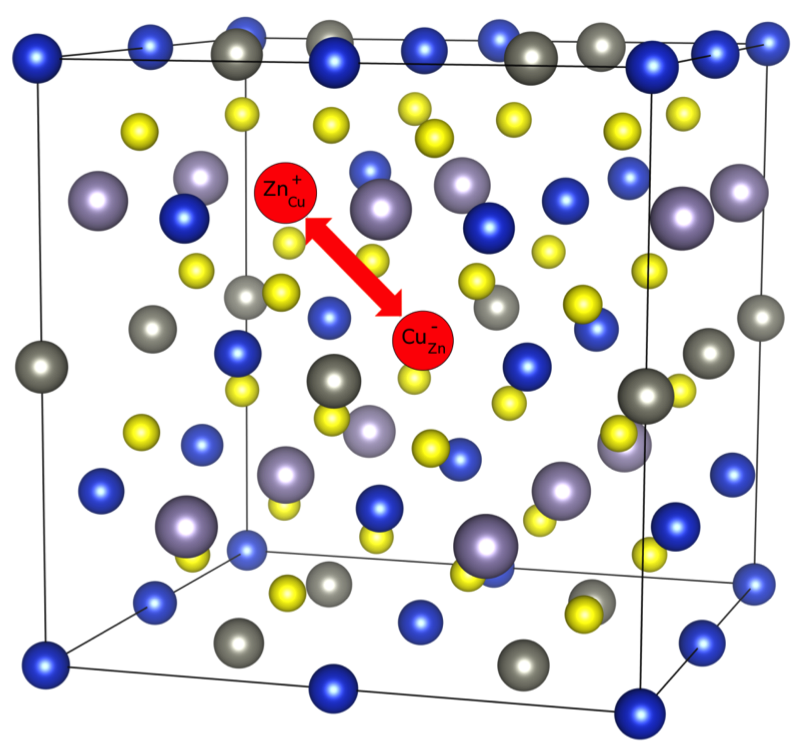
\includegraphics[width=0.5\textwidth]{figures/Cu-Zn_defect.png}
    \caption{64 atom supercell of {\CZTS} showing a substitution of Cu and Zn ions that results in the formation of the nearest neighbour antisite defect pair.}
  \label{Cu-Zn_defect}
\end{figure}

For our calculations of the formation energy of the nearest-neighbour [$Cu_{Zn}^- + Zn_{Cu}^+$] defect pair (shown in figure \ref{Cu-Zn_defect}), we make use of the Heyd-Scuseria-Ernzerhof (HSE06) hybrid-functional \cite{HSE} for the exchange-correlation functional as implemented in the Vienna Ab-initio Simulation Package (VASP) \cite{VASP}. This functional mixes 25\% of screened Hartree-Fock exchange to the Perdew-Burke-Ernzerhof (PBE) exchange functional \cite{PBE}. Projector augmented-wave potentials \cite{PAW} were used to describe the core electrons with an energy cut-off of 500 eV for the plane-wave basis set. Calculations were initially performed at the gamma point (a 1x1x1 \textit{k}-point mesh) until forces on the ions converged to within 0.01 eV/ $\AA$. 
A single geometry step was then performed with a 2x2x2 \textit{k}-point mesh centred on the gamma point as these parameters were found to be sufficient for the total energy to converge to within $<$2 meV  per atom with respect to increased plane-wave cut-off energy and for the external pressure to be $<$1 kbar. However, performing the full calculation with a 2x2x2 \textit{k}-point mesh was found to be too computationally expensive. Data for the convergence test is given is table \ref{conv_test}. From our calculation, we predict a defect formation energy of 0.30 eV.
\begin{table}[h]
\centering
\begin{tabular}{c|l|l|l|l}
Cut-off energy (eV) & \textit{k}-points & Total energy, E (eV) 
& \multicolumn{1}{|p{2cm}|}{ \centering External \\ pressure (kbar)} & dE per atom (meV)\\
\cline{1-5}
300 & $1\times1\times1$ & -305.53 & -174.59 & \\
350 & $1\times1\times1$ &  -306.95 & -23.86 & - 22.12\\
400 & $1\times1\times1$ &  -307.49 & 8.21 & - 8.47\\
450 & $1\times1\times1$ & -307.08 & 5.71 & 6.33\\
500 & $1\times1\times1$ & -307.20 & 4.02 & - 1.87\\
300 & $2\times2\times2$ & -306.76 & -180.97 & \\
500 & $2\times2\times2$ & -308.72 & -0.08 & \\
\end{tabular}
\caption{Convergence tests performed on the perfect CZTS supercell with various plane wave cut-off energies for the basis set and number of \textit{k}-points in the sampling where dE is the difference in the total energy obtained as the cut-off energy for the plane-wave basis set is increased in increments of 50 eV.}
\label{conv_test}
\end{table}

When defect concentrations are less than 1\%, it is usually assumed that the system is in the dilute defect limit where defects can be considered to be non-interacting. Using statistical thermodynamics for point defects, an expression for the equilibrium concentration of point defects as a function of temperature can be obtained \cite{thermodynamics}. This is shown in equation \ref{defect_conc}, where N is the number of sites, $\Delta H$ is the defect formation energy, $k_B$ is the Boltzmann constant and T is the temperature of the system.
\begin{equation} \label{defect_conc}
n = Ne^{\frac{-\Delta H}{k_BT}}
\end{equation}
The probability of defect formation as a function of temperature is given by the exponential expression in equation \ref{defect_conc}. The defect formation energy from the DFT calculations were halved to take an average of the formation energy per defect during the formation of an antisite pair before being inserted into this expression. This is plotted against temperature in figure \ref{Cu-Zn_eqm_conc}. 
\begin{figure}[h!]
  \centering
    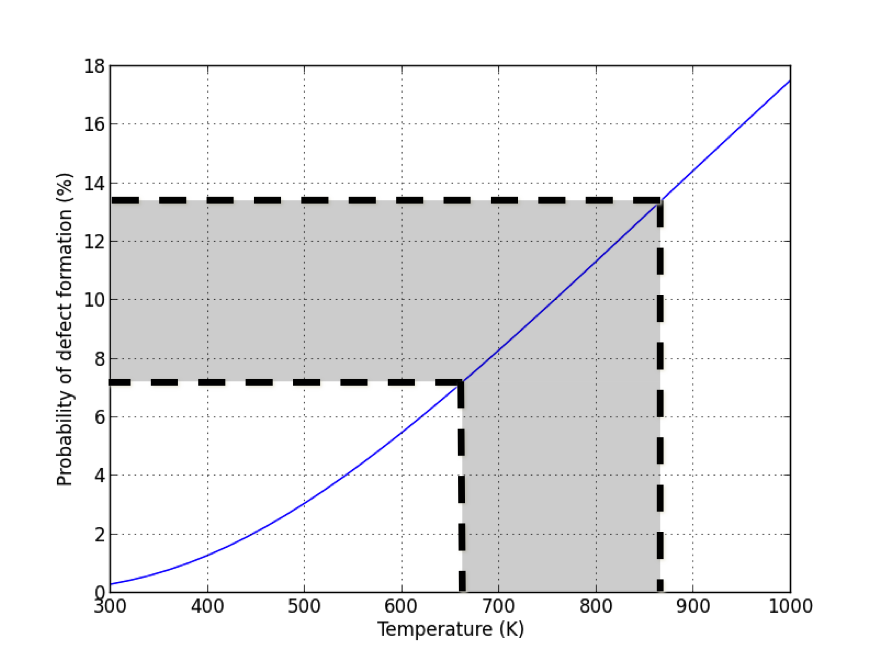
\includegraphics[width=0.9\textwidth]{figures/Cu-Zn_eqm_conc.png}
    \caption{Probability of nearest neighbour [$Cu_{Zn}^- + Zn_{Cu}^+$] defect formation as a function of temperature based on the equilibrium defect concentration from classical thermodynamics. The shaded region indicates typical annealing temperatures used in the synthesis of {\CZTS}.}
  \label{Cu-Zn_eqm_conc}
\end{figure}
It can be seen from figure \ref{Cu-Zn_eqm_conc} that the probability of defect formation at a typical annealing temperatures is approximately 7-13\%.
It was also found that, compared to the undefective system, there was a decrease in the separation of the antisite defects of 3.84$\AA$ to 3.82$\AA$ after the geometry optimization. This effect could be due to a Coulombic attraction between the two antisite defects.
The point defects (the $Cu_{Zn}^-$ and $Zn_{Cu}^+$ antisites) form the defect complex [$Cu_{Zn}^- + Zn_{Cu}^+$]. The point defects become associated with one another due to a Coulomb interaction between the effective +1 and -1 charge that results from substituting species with a +1 charge with a species with a +2 charge and vice versa. This, in addition to the high equilibrium concentrations of antisite defects predicted, suggests that it is not sufficient to consider the $Cu_{Zn}^-$ and $Zn_{Cu}^+$ antisites as non-interacting point defects and that we must instead consider a system of interacting defects.
 We aim to do this through our Monte Carlo simulations of thermodynamic disorder, which are discussed in section \ref{MC_section}.